
\section{Introduction}
Due to factors like non-ideal lighting, lack of texture and sensor noise of the smartphone, the obtained point cloud typically has noise and incompletions, with the points distributed around the `true' surface.
 Techniques like Screened Poisson reconstruction or the depth map fusion strategy of \cite{hernandez2015near} either return meshes with a lot of surface noise or extremely smoothed out details, depending on the regularization used (see Fig. \ref{fig:mesh_comp}). Further, for the reconstructed mesh to be of use in further downstream tasks such as animation, bio-metrics or as input to a learning algorithm, it is extremely desirable for the meshes to have a consistent topology. 
 \begin{figure}[t]
\begin{center}
   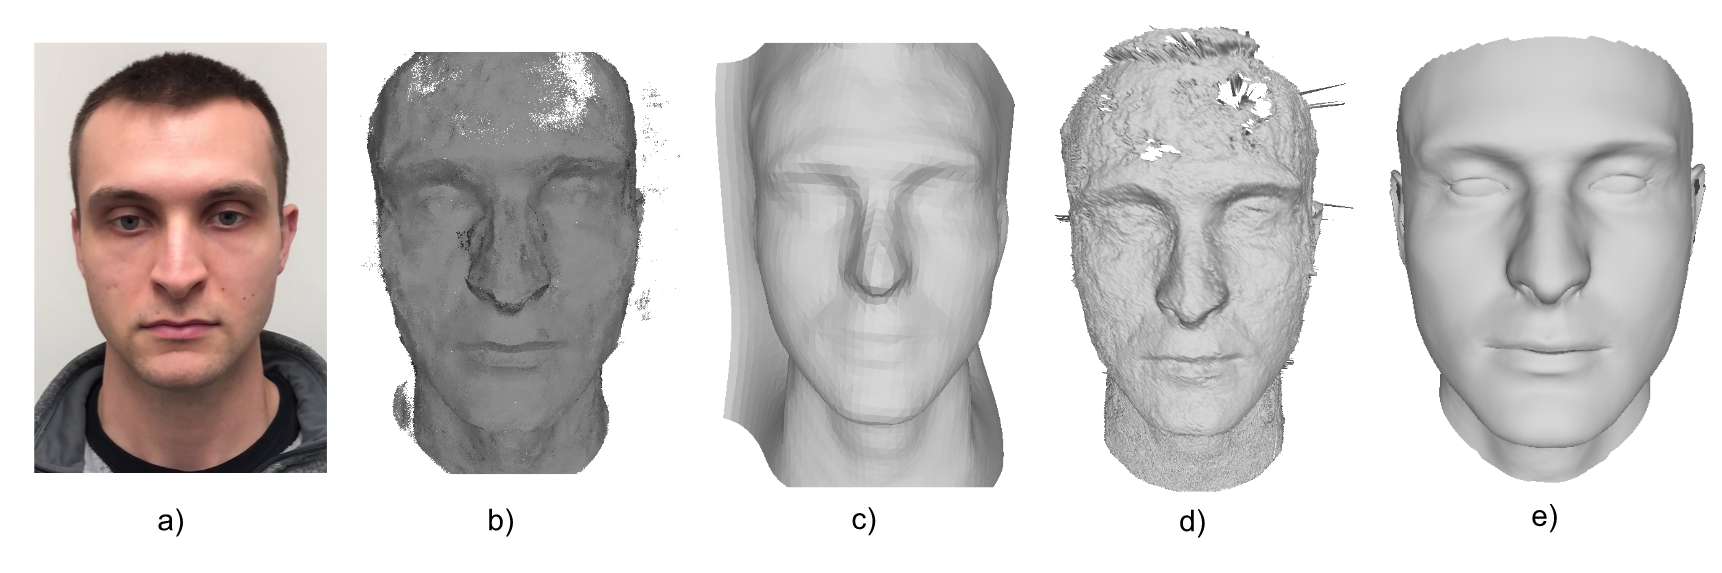
\includegraphics[width=0.95\linewidth]{images/meshing_compare.png}
\end{center}
   \caption{Comparison of mesh generation methods a) Sample image. b) Generated point cloud (\ref{sec:pcl}) c) \cite{kazhdan2013screened} can fill in gaps in the point cloud but at the cost of overly smooth meshes. d) Depth fusion method of \cite{hernandez2015near} can preserve details, but is unable to handle missing data. e) Our approach reconstructs meshes with consistent topology and correspondence between vertices, while capturing details of the point cloud and being robust to noise and missing data. }
\label{fig:mesh_comp}
\end{figure}

 Statistical ICP inspired techniques have proposed fitting a 3DMM to a point cloud \cite{schneider2009fitting,bazik2017robust,blanz2004statistical} in the past. However, they often assume that the point cloud is from an RGB-D sensor and so has a single, `clean' surface. Further, fitting a 3DMM defeats the purpose of not being constrained to an existing linear basis of shape.
 We thus adapt the non-rigid mesh fitting algorithm of \cite{amberg2007optimal}, originally proposed for registering template meshes to 3D scanner data, to deform a template using a combination of constraints given by the point cloud, landmarks, mesh stiffness and edge constraints. 
 
 
 \section{Point cloud constraints}
 The primary constraint for the mesh deformation comes from the 3D information captured in the point cloud.
 While well-studied techniques exist to register a template mesh to a 3D scanned mesh \cite{amberg2007optimal}, registering a mesh to point clouds of the sort obtained from multi-view stereo techniques is more challenging. For example, simply fitting each vertex to its nearest-neighbor in the point cloud will cause the mesh to become extremely noisy, as there will be many outlier points.
 
To address this, we take advantage of the fact that for a template mesh, the vertex normals can be easily estimated. For each vertex, we select the points in its neighborhood, and for each point, we calculate its perpendicular distance to the normal of the vertex. Points within a small threshold distance are accepted while the rest are rejected (see Fig. \ref{fig:mesh_fit_pcl}. 
 
 For each vertex on the template mesh we obtain its desired location in 3D as the median of the accepted points.
 
\begin{figure}[t]
\begin{center}
   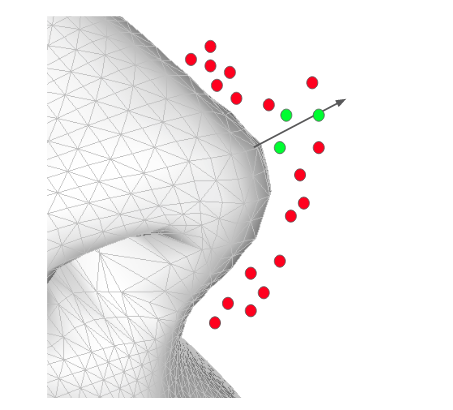
\includegraphics[width=0.7\linewidth]{images/mesh_fit_pcl.png}
\end{center}
   \caption{Exaggerated view of the point cloud constraints. For each vertex, the set of points within a small threshold of its normal (in green here) are found and their median used as the target 3D coordinate for the vertex. }
\label{fig:mesh_fit_pcl}
\end{figure}

 
 \section{Landmark constraints}

 The second source of information are the 68 2D landmarks obtained using the automatic landmarking solution of \cite{baltrusaitis2018openface}. Landmarks are important for global alignment and scaling of the mesh, as well as ensuring all the reconstructed meshes are in semantic correspondence.
 
 For the set of frames for which the landmarks have been annotated with high confidence by the tracker (typically close to frontal poses), we solve for the 3D locations of the landmarks by minimizing geometric reprojection error, 
 \begin{equation}
    E_{X_{j}} = \sum_{i} \sum_{j} d(\pi (\theta_{i},X_{j}),x_{ij})^2
\end{equation}
Where $\theta_i$ is the $i$-th camera's pose, $X_{j}$ is the $j$-th landmark's coordinates in 3D, and $x_{ij}$ is the 2D coordinate of the landmark returned by the landmark tracker for the $i$-th frame. For our purposes, we ignore the 18 landmarks corresponding to the face contour, and use the remaining 50 landmarks as constraints for the corresponding 3D vertices.

Historically, most landmark trackers have focused only on these 68 keypoints. As a consequence, many reconstruction techniques either focus only on reconstructing the frontal face region, or generate a full mesh but evaluate only on the frontal section. Ears and the side facial regions have mostly been ignored in previous works. Even learning-based face alignment techniques do not do well on the ears, as the underlying training data is based on the annotation/detection of these 68 landmarks.

To explicitly address this, we make use of a recent dataset of `in-the-wild' ear images annotated with bounding boxes and landmarks \cite{zhou2017deformable}. We first train the deep object detection model of Redmon \etal \cite{redmon2017yolo9000} for a single `ear' class. We then train an ensemble of regression trees \cite{kazemi2014one} for predicting landmarks using the bounding box detection as input. As seen in Fig \ref{fig:ear_lm_and_edges}, despite the limited training data size, we are able to achieve impressive robustness and accuracy in the landmark detection. We use a subset of the landmarks corresponding to the outer contour of the ear as additional landmark constraints in our mesh fitting. To the best of our knowledge, ours is the first face reconstruction method to explicitly address the ears, which in turn improves overall accuracy and metrics like the width of the face.

\begin{figure}[t]
\begin{center}
   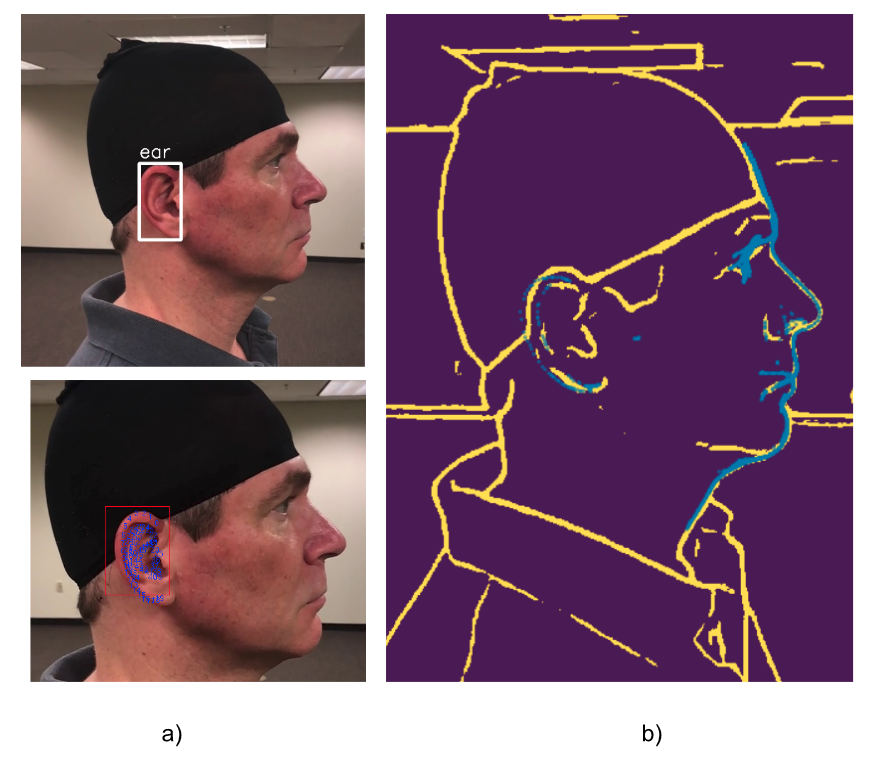
\includegraphics[width=0.8\linewidth]{images/ear_lm_and_edges.png}
\end{center}
   \caption{ a) We train a bounding box regressor (above) and landmark detector (below) specifically for ears. This improves our reconstruction's overall accuracy while allowing us to capture ear size and contour. b) Visualization of edge constraints. Image edges in yellow, mesh vertices corresponding to edges projected in blue. Note that mesh vertices fit the ear well because of the ear landmark detection. }
\label{fig:ear_lm_and_edges}
\end{figure}





\section{Edge constraints}
Silhouette constraints have shown to be powerful cues in recent 3D reconstruction literature \cite{alldieck2018detailed,bas2016fitting}. For faces, views that are close to profile are particularly informative. However, since many single and multi-view approaches rely on landmarking for camera pose estimation, they fail to make use of silhouettes beyond a certain angle. By solving for the camera poses independently of landmarking, we can actually make use of extreme profile views. This proves to be helpful in capturing challenging areas for face reconstruction algorithms, such as the nose, lips and lower chin/neck region.
We use a combination of Z-buffering \cite{Foley1990ComputerG} and backface-culling  to estimate vertices that project an edge onto a given view. To find the corresponding edges in the RGB image, we use the Structured Forests edge detection approach proposed in \cite{dollar2013structured}. For each vertex projecting an edge in the frame, its nearest neighbor is found in the edge map. This corresponding point is back-projected in 3D to obtain a `target' location for the vertex in 3D.


 \section{Non-Rigid Iterative Closest Points}
 With the combination of the cues from the point cloud, landmarks, and silhouettes, we obtain a set of constraints that we wish to use to deform the template mesh. For a template mesh M of fixed topology (V, E), this can be written as a weighted sum of energies we wish to minimize: 
 $$ \arg \min_{V}  E_{pcl} + \alpha E_{lms} + \beta E_{edges} +  \gamma E_{reg} $$
where $E_{reg}$ is a regularization energy arising from the mesh topology that restricts connected vertices to deform similarly. This system can naturally be expressed in the iterative linear system-based non-rigid mesh registration algorithm proposed by Amberg \etal \cite{amberg2007optimal}. 
 
 At each iteration, a linear system of the form $\mathbf{A}\mathbf{X} = \mathbf{B}$ is solved, where $\mathbf{X}$ is a $4n\times3$ matrix, containing the per-vertex 3x4 affine transform matrix. The matrix $\mathbf{A}$ captures information of the source template in terms of the mesh connectivity and vertex locations. The mesh connectivity acts as an adjustable `stiffness' regularization, which controls how much neighboring vertices can move with respect to each other. The matrix $\mathbf{B}$ contains the corresponding `target' locations in 3D, such as those obtained from the point cloud, landmarks and edges.\\
 %%to edit
 
 Where $W := diag(w_1, \dots, w_n)$, D is a sparse matrix mapping the
$4n\times3$ matrix of unknowns $X$ onto displaced source vertices.

For the stiffness item, we define a node-arc incidence matrix $M$. If
edge $r$ connects the vertices $(i, j)$ and $i<j$, the nonzero entries
of $M$ in row $r$ are $M_{ri} = −1$ and $M_{rj} = 1$. Then the item
can be rewritten as:

\begin{equation}
  E_s(X) := {\| (M \otimes G)X \|}_F^2
\end{equation}

Similarly, the rest two item can also be rewritten in the form of

\begin{equation}
  E_l(X) := {\| D_LX - U_L \|}_F^2
\end{equation}

\begin{equation}
  E_m(X) := {\| DX - U_m \|}_F^2
\end{equation}

Now, the original cost function becomes a quadratic function:

\begin{equation}
  \begin{array}{lcl} 
    E(X) & = & {\left\Vert \left[ \begin{array}{c} WD \\ \alpha M \otimes G \\ \beta D_L \\ \gamma D \end{array} \right] X - \left[ \begin{array}{c} WU \\  0 \\  \beta U_L \\ \gamma U_m \end{array} \right] \right\Vert_F^2} \\
     
    & & \\
    
  & = & \left\Vert AX - B \right\Vert_F^2
  \end{array} 
\end{equation}

which is a typical linear least square problem. And $E(X)$ takes on its
minimum at $X = (A^TA)^{-1}A^TB$.  Thus, For each iteration, given
fixed correspondences and coefficents, we could determine the optimal
deformation quickly. We use sksparse's cholesky decomposition functionality to do this inversion efficiently.

%%
 
 
 The mesh stiffness and the weights of the landmarks are gradually decreased, gradually moving from global stretching to local, data-driven deformations. After every few iterations, the point cloud and edge constraints are recalculated using the current locations of the vertices. For further details, we refer the reader to the original paper \cite{amberg2007optimal}. For our template, we use the Basel 3DMM mesh \cite{blanz1999morphable}, simply because of its prevalence as an input or output of several face reconstruction algorithms.